\chapter{Estudo de simulação}

%=====================================================

Com o objetivo de avaliar o poder do teste Wald em testes de hipóteses sobre parâmetros de McGLMs, foram executados estudos de simulação. Nestas simulações avaliamos o comportamento da proposta para três distribuições de probabilidade: Normal, Poisson e Bernoulli. Simulamos cenários univariados e também trivariados com diferentes tamanhos amostrais para verificar as propriedades dos testes sobre parâmetros de regressão, dispersão e potência.

Para simular conjuntos de dados univariados foram usadas bibliotecas padrões do R. Para simular conjuntos de dados com múltiplas respostas seguindo distribuição Normal, foi usada a biblioteca R \emph{mvtnorm} \citep{mvtnorm1}, \citep{mvtnorm2}. Para as outras distribuições foi utilizado o método NORTA \citep{cario1997modeling} implementado na biblioteca R \emph{NORTARA} \citep{nortara}.

\section{Parâmetros de regressão}

Para avaliação de hipóteses sobre parâmetros de regressão foram considerados tamanhos amostrais de 50, 100, 250, 500 e 1000. Foram gerados 500 conjuntos de dados para cada tamanho amostral simulando uma situação com uma variável explicativa categórica de 4 níveis. Para distribuição Normal os parâmetros de regressão usados foram: $\beta_0 = 5$, $\beta_1 = 0$, $\beta_2 = 0$, $\beta_3 = 0$. Para a distribuição Poisson os parâmetros de regressão usados foram: $\beta_0 = 2,3$, $\beta_1 = 0$, $\beta_2 = 0$, $\beta_3 = 0$. E para a distribuição Bernoulli os parâmetros de regressão usados foram: $\beta_0 = 0,5$, $\beta_1 = 0$, $\beta_2 = 0$, $\beta_3 = 0$. Os valores foram escolhidos de tal modo que o coeficiente de variação para distribuição Normal fosse de 20\%, as contagens para Poisson fossem próximas de 10 e a probabilidade de sucesso da Bernoulli fosse aproximadamente 0,6. Foram avaliados cenários univariados e trivariados com estas características. Para os cenários trivariados, existem 4 parâmetros por resposta que seguem as configurações descritas. Para cada amostra gerada foi ajustado um McGLM nos quais as funções de ligação e variância para cada distribuição são apresentadas na \autoref{tab:link_var}. 

\begin{table}[H]
\centering
\begin{tabular}{ccc}
\hline
Distribuição & Função de ligação & Função de variância \\ \hline
Normal       & Identidade        & Constante           \\
Poisson      & Logarítmica       & Tweedie             \\
Bernoulli    & Logito            & Binomial            \\ \hline
\end{tabular}
\caption{Funções de ligação e variância utilizadas nos modelos para cada distribuição simulada.}
\label{tab:link_var}
\end{table}

Em todos os casos o preditor matricial para a matriz de variância e covariância foi especificado de forma a explicitar que as observações são independentes dentro de cada resposta. A correlação entre respostas no caso trivariado é dada pela matriz $\Sigma_b$ descrita na \autoref{eq:correlacao}.

\begin{equation} \label{eq:correlacao}
\Sigma_b = 
\begin{bmatrix}
1    & 0,75 & 0,5  \\
0,75 & 1    & 0,25 \\
0,5  & 0,25 & 1    \\
\end{bmatrix}
\end{equation}

Com os modelos ajustados, o procedimento consistiu em variar as hipóteses testadas sobre os parâmetros simulados. Consideramos 20 diferentes hipóteses baseadas em um decréscimo em $\beta_0$ e distribuição deste decréscimo nos demais $\beta$s da hipótese nula. O decréscimo para respostas seguindo distribuição Normal foi de 0,15; para distribuição Poisson o decréscimo foi de 0,05; e para distribuição Bernoulli o decréscimo foi de 0,25. Estes valores foram escolhidos levando em conta o o afastamento desejado das hipóteses testadas na escala da resposta e é importante notar que estes valores são diferentes devido ao impacto da função de ligação usada em cada configuração de modelo e também devido às propriedades dos parâmetros das distribuições.

Para cada ponto avaliamos o percentual de rejeição da hipótese nula. A ideia é verificar o que ocorre quando afastamos as hipóteses nulas dos reais valores dos parâmetros. Espera-se que no primeiro ponto haja um percentual de rejeição baixo, pois a hipótese nula corresponde aos reais valores dos parâmetros. Para os demais pontos espera-se que o percentual de rejeição aumente gradativamente, pois as hipóteses afastam-se cada vez mais dos valores originalmente simulados. 

\textbf{As hipóteses testadas em cada cenário estão disponíveis no apêndice desta dissertação.}
 
Para representar graficamente os resultados tomamos a distância euclideana de cada vetor de hipóteses com relação ao vetor usado para simular os dados. Adicionalmente dividimos o vetor de distâncias pela maior distância para obter distâncias padronizadas entre 0 e 1, independente dos parâmetros de regressão. Os resultados são apresentados na \autoref{fig:betas}.

\begin{figure}[H]
\centering
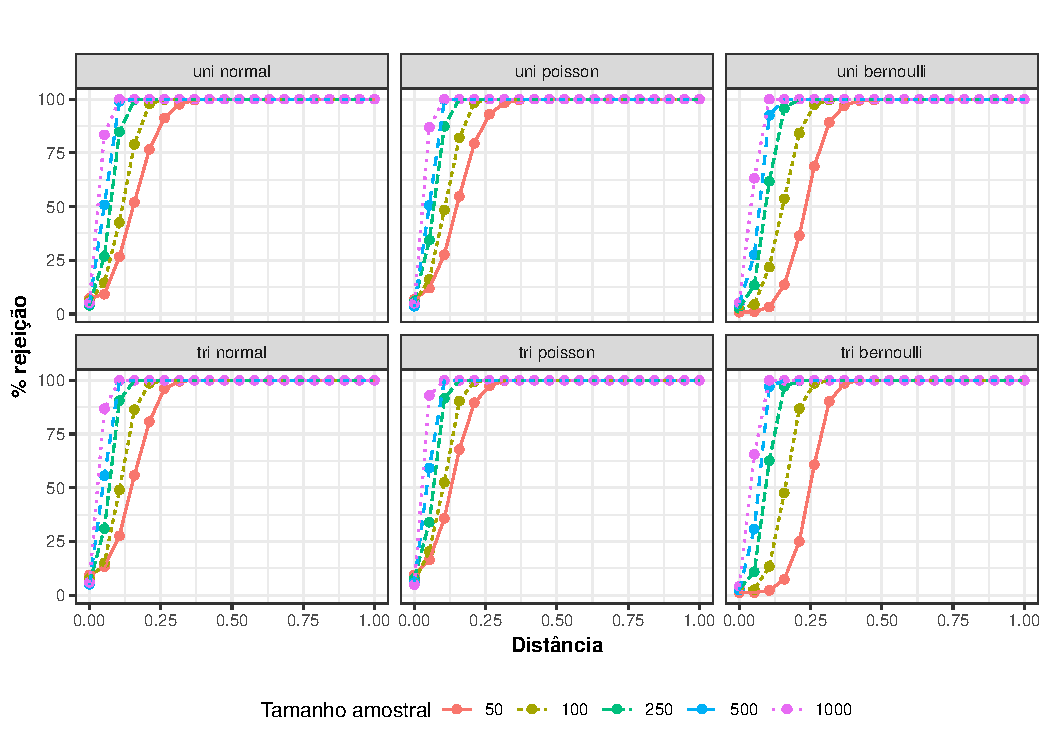
\includegraphics[width=15cm]{/home/lacf14/msc/4_dissertacao/6-simulacao/betas.pdf}
\caption{Resultados do estudo de simulação para os parâmetros de regressão.}
\label{fig:betas}
\end{figure}

De modo geral, quanto mais distante a hipótese é dos valores inicialmente simulados, maior é o percentual de rejeição. Como esperado, os menores percentuais foram observados na hipótese igual aos valores simulados. Nos cenários univariados o percentual de rejeição foi próximo de 5\% quando a hipótese era igual aos valores simulados mesmo com tamanhos amostrais reduzidos. Para os cenários trivariados, no menor tamanho amostral avaliado, o percentual de rejeição não excedeu 10\% e em tamanhos amostrais iguais a 500 o percentual de rejeição foi próximo de 5\%. Também como esperado, foi possível verificar que conforme aumenta-se o tamanho amostral, o percentual de rejeição aumenta para hipóteses pouco diferentes dos valores simulados dos parâmetros.

\section{Parâmetros de dispersão}

Para avaliação de hipóteses sobre parâmetros de dispersão foram considerados os mesmos tamanhos amostrais: 50, 100, 250, 500 e 1000. Contudo, os conjuntos de dados simulam uma situação em que cada unidade amostral fornece 5 medidas ao conjunto de dados. Foram gerados 500 conjuntos de dados para cada tamanho amostral e distribuição. Para distribuição Normal foram simulados vetores com média 5 e desvio padrão igual a 1. Para distribuição Poisson foram simuladas contagens com taxa igual a 10. Para distribuição Bernoulli foram simulados vetores de uma variável dicotômica com probabilidade de sucesso igual a 0,6.

Em todos os casos, os parâmetros de dispersão para gerar os conjuntos de dados foram fixados em $\tau_0 = 1$, $\tau_1 = 0$ e não foi incluído efeito de variáveis explicativas. Foram avaliados cenários univariados e trivariados com estas características. Para cada amostra gerada foi ajustado um McGLM com funções de ligação e variância tal como descrito na \autoref{tab:link_var}. Nos cenários trivariados a correlação entre respostas é dada pela \autoref{eq:correlacao}.

Neste caso, como o objetivo é avaliar a correlação dentro das respostas, é necessário especificar um preditor matricial. O objetivo é testar hipóteses sobre os parâmetros de dispersão associados a este preditor matricial. 

Com os modelos ajustados, o procedimento consistiu em variar as hipóteses testadas sobre os parâmetros simulados. Consideramos 20 diferentes hipóteses baseadas em um decréscimo sucessivo de 0,02 em $\tau_0$ e acréscimo de 0,02 em $\tau_1$ para cada hipótese nula testada. Para cada ponto avaliamos o percentual de rejeição da hipótese nula. A ideia é afastar sucessivamente a hipótese dos valores simulados e avaliar se conforme afastamos a hipótese dos valores verdadeiros, o percentual de rejeição aumenta. 

\textbf{As hipóteses testadas estão disponíveis no apêncice.}

Do mesmo modo que foi feito para os parâmetros de regressão, foi tomada a distância euclideana de cada vetor de hipóteses com relação ao vetor usado para simular os dados; e o vetor de distâncias foi padronizado para obter distâncias entre 0 e 1. Os resultados são apresentados na \autoref{fig:taus}.

\begin{figure}[H]
\centering
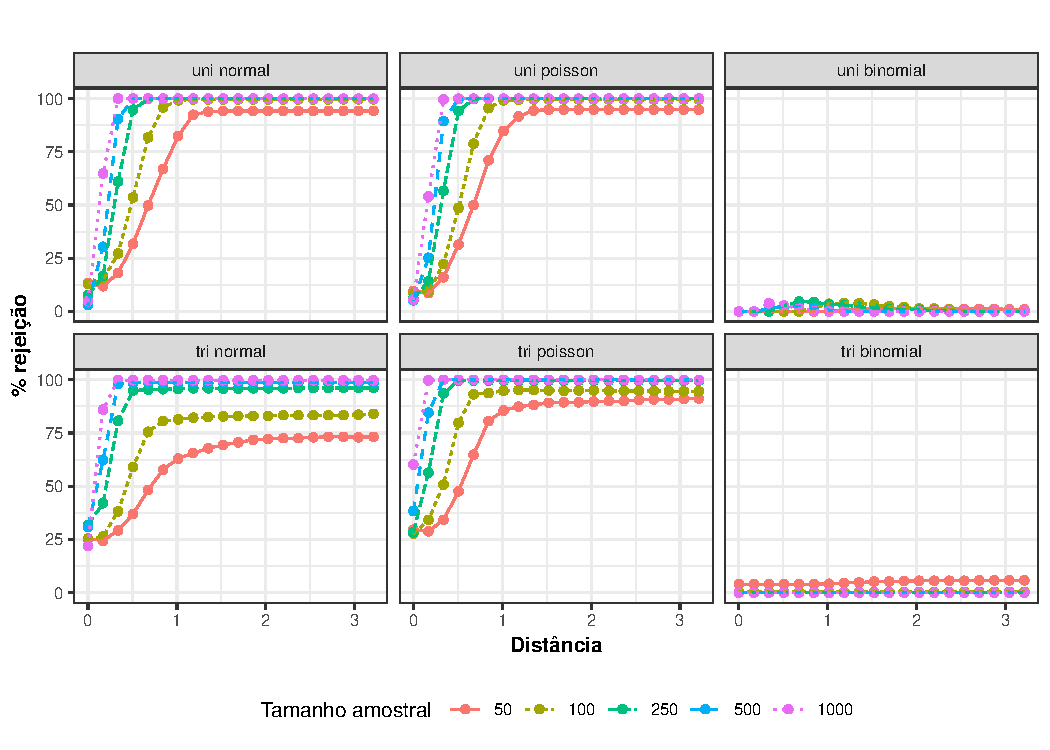
\includegraphics[width=15cm]{/home/lacf14/msc/4_dissertacao/6-simulacao/taus.pdf}
\caption{Resultados do estudo de simulação para os parâmetros de dispersão.}
\label{fig:taus}
\end{figure}

Assim como observado para os parâmetros de regressão, o comportamento dos gráficos mostra que, quanto mais distante a hipótese é dos valores inicialmente simulados, maior é o percentual de rejeição, e os menores percentuais são observados em hipóteses próximas aos valores simulados. Na primeira hipótese testada, para os cenários univariados, percentuais de rejeição próximos a 8\% na primeira hipótese foram observados no menor tamanho amostral avaliado. A partir de tamanhos amostrais iguais a 250 o percentual de rejeição foi próximo de 5\%. Já para os casos trivariados, no menor tamanho amostral, o percentual de rejeição excedia 10\% no menor tamanho amostral; para tamanhos amostrais maiores, os percentuais ficaram em torno de 7\%. Também verificou-se para parâmetros de dispersão que conforme aumenta-se o tamanho amostral, o percentual de rejeição aumenta para hipóteses pouco diferentes dos valores simulados dos parâmetros.

\section{Parâmetros de potência}

Para avaliação de hipóteses sobre parâmetros de potência foram novamente considerados tamanhos amostrais de 50, 100, 250, 500 e 1000. Foram gerados 500 conjuntos de dados para cada tamanho amostral simulando uma situação com uma variável explicativa categórica de 2 níveis. Para distribuição Normal os parâmetros de regressão usados foram: $\beta_0 = 3$ e $\beta_1 = 2$. Para a distribuição Poisson os parâmetros de regressão usados foram: $\beta_0 = 1,3$ e $\beta_1 = 0,7$. E para a distribuição Bernoulli os parâmetros de regressão usados foram: $\beta_0 = 0,35$ e $\beta_1 = 0,15$. Os valores foram escolhidos de tal modo que haja um parâmetro de regressão com efeito significativo para que seja possível estimar os parâmetros de potência. Foram avaliados cenários univariados e trivariados com estas características.

A correlação entre respostas no caso trivariado é dada pela matriz $\Sigma_b$ descrita na \autoref{eq:correlacao}. Para cada amostra gerada foi ajustado um McGLM em que para todos os casos o preditor matricial foi especificado de forma a explicitar que as observações são independentes dentro de cada resposta.

Similar ao que foi feito para parâmetros de regressão e dispersão, o procedimento consistiu em variar as hipóteses testadas sobre os parâmetros simulados. Nestas configurações, espera-se que o parâmetro de potência seja 0, 1 e 1 para as distribuições Normal, Poisson e Bernoulli, respectivamente. Para avaliar o teste, consideramos 20 diferentes hipóteses baseadas em um acréscimo sucessivo de $2/20$ para cada hipótese nula testeda. Para cada ponto avaliamos o percentual de rejeição da hipótese nula. Tal como nos casos anteriores espera-se que, afastando os valores da hipótese dos valores verdadeiros, o número de rejeições cresça. As hipóteses testadas são mostradas na \autoref{tab:th_p}.

\begin{table}[H]
\centering
\begin{tabular}{cccc}
\hline
          & Normal & Poisson & Bernoulli \\ \hline
$H_{01}$  & 0      & 1       & 1         \\
$H_{02}$  & 0,1    & 1,1     & 1,1       \\
$H_{03}$  & 0,2    & 1,2     & 1,2       \\
$H_{04}$  & 0,3    & 1,3     & 1,3       \\
$H_{05}$  & 0,4    & 1,4     & 1,4       \\
$H_{06}$  & 0,5    & 1,5     & 1,5       \\
$H_{07}$  & 0,6    & 1,6     & 1,6       \\
$H_{08}$  & 0,7    & 1,7     & 1,7       \\
$H_{09}$  & 0,8    & 1,8     & 1,8       \\
$H_{010}$ & 0,9    & 1,9     & 1,9       \\
$H_{011}$ & 1      & 2       & 2         \\
$H_{012}$ & 1,1    & 2,1     & 2,1       \\
$H_{013}$ & 1,2    & 2,2     & 2,2       \\
$H_{014}$ & 1,3    & 2,3     & 2,3       \\
$H_{015}$ & 1,4    & 2,4     & 2,4       \\
$H_{016}$ & 1,5    & 2,5     & 2,5       \\
$H_{017}$ & 1,6    & 2,6     & 2,6       \\
$H_{018}$ & 1,7    & 2,7     & 2,7       \\
$H_{019}$ & 1,8    & 2,8     & 2,8       \\
$H_{020}$ & 1,9    & 2,9     & 2,9       \\ \hline
\end{tabular}
\caption{Hipóteses testadas para parâmetros de potência para cada distribuição simulada.}
\label{tab:th_p}
\end{table}


Da mesma forma que o realizado para o estudo sobre parâmetros de regressão e dispersão, tomamos a distância euclideana de cada vetor de hipóteses com relação ao vetor usado para simular os dados e padronizamos o vetor. Os resultados são apresentados na \autoref{fig:ps}.

\begin{figure}[H]
\centering
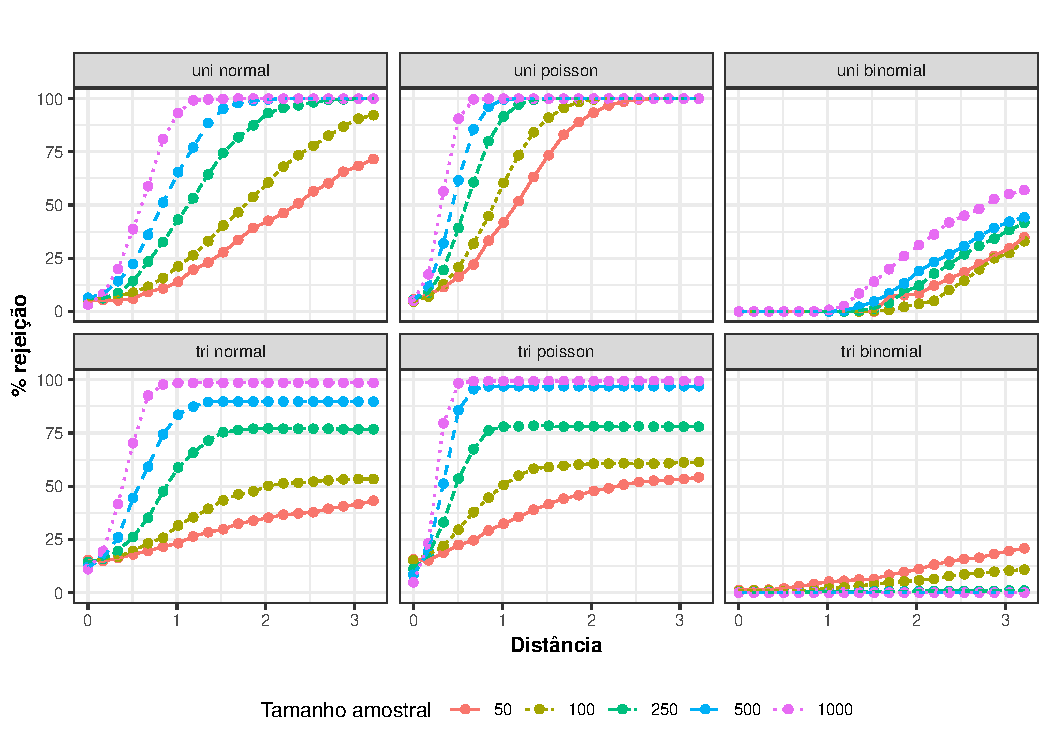
\includegraphics[width=15cm]{/home/lacf14/msc/4_dissertacao/6-simulacao/ps_old.pdf}
\caption{Resultados do estudo de simulação para os parâmetros de potência.}
\label{fig:ps}
\end{figure}

Os resultados para os parâmetros de potência nos casos univariados com distribuição Normal e Poisson se mostraram bastante satisfatórios, com percentuais de rejeição próximos a 5\% na hipótese igual aos valores simulados com percentual de rejeição crescente nas hipóteses mais afastadas. Tal como ocorreu para os parâmetros de regressão há um desempenho inferior para distribuição Bernoulli no caso univariado indicando que existe a necessidade de tamanhos amostrais maiores para realização dos testes.

Para os cenários trivariados com distribuição Normal e Poisson, o percentual de rejeição cresce a medida que afastamos as hipóteses dos valores simulados, contudo o percentual de rejeição na hipótese igual aos valores simulados é próximo de 15\%. Já para distribuição Bernoulli no cenário trivariado não foram obtidos resultados satisfatórios.

%=====================================================

\textbf{TODO}

\begin{itemize}

  \item \textbf{COLOCAR TABELAS COM HIPÓTESES TESTADAS NO APENDICE}

  \item \textbf{VER COM O WAGNER SE A JUSTIFICATIVA DO TAMANHO DO PASSO PARA HIPÓTESES DOS BETAS ESTÁ SUFICIENTE}

  \item \textbf{COMO PROCEDER COM OS PARAMETROS DE POTENCIA}

\end{itemize}

%=====================================================